\documentclass{../../myassignment}

\usepackage{array}

\courselabel{IN1030}
\exercisesheet{Oblig 2}{Bruk og brukerundersøkelser}

\usepackage{xcolor}
\definecolor{block-gray}{gray}{0.85}

\usepackage{environ}

\NewEnviron{myblock}
{\colorbox{block-gray}{%
\parbox{\dimexpr\linewidth-2\fboxsep\relax}{%
\small\addtolength{\leftskip}{5mm}
\addtolength{\rightskip}{5mm}
\BODY}}
}

\renewcommand{\quote}{\myblock}
\renewcommand{\endquote}{\endmyblock}

\begin{document}
	\subsection*{Oppgave 1 --- Observasjon av bruk}
	\paragraph*{a)}

	% Planlegg datainnsamlingen. Beskriv følgende:
		% Hva du forventer å finne ut ved å studere interaksjonen mellom en bruker og den digitale løsningen, og hvem du tror faller innenfor målgruppen til systemet?
		Ved {\aa} studere interaksjonen mellom flere brukere av det eksisterende Vy-systemet og dens maskiner forventer jeg {\aa} finne ut hvordan folk generelt sett tiln{\ae}rmer seg en togstasjon. Jeg har allerede opplevd selv at problemer allerede kan oppst{\aa} f{\o}r vi engang n{\aa}r det digitale punktet. Eksempler inkluderer at vi ikke vet hvor stedet ligger, ikke finner inngangen, eller ikke kjenner igjen maskinene. 

		I noen omstendigheter vet ikke brukeren om protokollene heller, og det finnes ingen lett tilgjenglige instrukser. Forskjellige aldersgrupper og forskjellige bakgrunner vil ha forskjellige problemer, og m{\aa}ter {\aa} l{\o}se disse problemene p{\aa}. Jeg {\o}nsker {\aa} f{\aa} et innblikk i disse grupperingene, og finne frem generiske l{\o}sninger og betraktninger man m{\aa} tenke p{\aa}.

		% Opp til 5 relevante oppgaver du vil be deltakeren om å utføre i systemet.
		\begin{itemize}
		\item[---] Kj{\o}pe en billett via datamaskin. 
		\item[---] Kj{\o}pe en billett ved en vilk{\aa}rlig og ukjent stasjon. 
		\item[---] Refundere en billett.
		\item[---] Finne frem fra en stasjon til en annen stasjon, uten aa bruke eksterne hjelpemidler (alts{\aa} ved {\aa} bare bruke Vy-tilbudte systemer). 
		\item[---] F{\aa} kontakt med en ansatt for {\aa} sp{\o}rre etter hjelp (toalettet? spr{\aa}khjelp? assistanse? {\dots}?)
		\end{itemize}


		% Deltakeren. Er hun/han en del av målgruppener
		Deltakeren jeg har valgt er en del av den yngre m{\aa}lgruppen. Yngre mennesker er en del av fremtiden, og burde kanskje derfor bli prioritert n{\aa}r det gjelder innovasjon, men p{\aa} den andre siden s{\aa} er det gjerne de yngre gruppene som trenger minst hjelp. Det beste ville v{\ae}rt {\aa} sp{\o}rre flere ``typer'' mennesker, og f{\aa} et bredt innblikk av systemet. {\AA} ha muligheten til {\aa} gj{\o}re denne observasjonen i utlandet gir meg muligheten til {\aa} observere hvordan systemet fungerer her, for {\aa} s{\aa} sammenligne med systemet i Norge, og eventuelt se forskjellen mellom hvordan folk oppf{\o}rer seg annerledes her enn der.

		% Din relasjon til deltakeren. Hvordan tror du dette kan spille inn på dataen du samler inn?
		Siden jeg er ganske kjent med dev vedkomnmende deltageren ville det kanskje v{\ae}re lett {\aa} tenke seg at jeg vil forvrenge resultatene av observasjonen, men jeg er ganske vant med {\aa} v{\ae}re ekstern observat{\o}r uten {\aa} innblande meg. Desutten vil jeg informere om dette f{\o}r observasjonen, for {\aa} unng{\aa} innblanding.

		% Hvordan du vil registrere data under observasjonen, som for eksempel medpenn/papir, opptak av lyd, fotografier, video, annet?
		Jeg har tenkt {\aa} forklare gj{\o}rem{\aa}lene hver for seg, og filme diverse snutter som jeg videre analyserer hjemme. Jeg tror det vil v{\ae}re lettere {\aa} analysere detaljer i etterkant ved {\aa} kunne se ting om igjen, med god tid. Alternativet ville v{\ae}rt {\aa} skrive ting opp etterhvert som de skjer, eller bare bruke hukommelsen. Om deltageren ikke {\o}nsker {\aa} bli filmet vil jeg forbrede handligssekvens-tabellen i forkant, for {\aa} s{\aa} skrive fortl{\o}pende det jeg ser. 

		Konklusjonen og utdypelsen av analysen m{\aa} skje i etterkant uansett, men ikke alt for lenge etter, siden hukommelsen ogs{\aa} har et betydning i helheten.


	\newpage

	\paragraph*{b)}

	Personvern er en viktig del av integriteten til alle og enhver. {\AA} vite hvilken informasjon av en selv som blir brukt av andre er viktig for mange, og fra et filosofisk standspunkt ville det ver uetisk {\aa} bruke informasjon om andre uten deres modne, fullverdige, og frie sammtykelse. 

	Det er i tillegg p{\aa}krevd av alle land innenfor EU {\aa} f{\o}lge GDPR (General Data Protection Regulation), p{\aa}krevd siden 2018 med bakgrunn p{\aa} etiske prinsipper som tidligere ble brutt. {\AA} ikke f{\o}lge denne loven kan risikere selskapet store p{\aa}legg, og eventuelt bli lagt ned om ledelsen ikke tilrettelegger l{\o}sninger, og f{\o}lger disse.

	\paragraph*{c)}

	\begin{quote}
		Sammtykelse for student-observasjon\\

		Jeg, \_\_\_\_\_\_\_\_\_\_\_\_\_\_\_, godtar, forst{\aa}r, og samtykker med at mitt navn blir registrert i en del av unders{\o}kelsen som ble gjort den \_\_ februar i 2020. Denne informasjonen vil bli brukt til akademiske form{\aa}l som en del av en student-unders{\o}kelse, og vil ikke bli behandlet i en komersiell sammenheng.\\

		Ved {\aa} signerere dette dokumentet lar jeg Rolf Vidar Mazunki Hoksaas observere og ta opp det jeg gj{\o}r, for {\aa} videre analysere situasjonen, valgene, og omheng. Resultatene av observasjonen vil kunne bli publisert, enten med, eller uten mitt navn. Dette gj{\o}r jeg av min egen fri vilje, uten noen personlig gevinst, eller noen form for press. 

		\vspace{1cm}

		\_\_\_\_\_\_\_\_\_\_\_\_\_\_\_, Barcelona. \_\_. februar, 2020.

		\vspace{5mm}\hrule\vspace{5mm}
	
		Consentimiento para observaci\'on acad\'emica.\\

		Yo, Gissela Celi Castillo, acepto, entiendo, y consiento que mi nombre sea registrado como parte de una observaci\'on realizada el 9 de febrero en 2020. Esta informaci\'on ser\'a utilizada como parte de un estudio sin fines econ\'omicos, y no ser\'a comercializado.\\

		Al firmar este documento, permito que Rolf Vidar Mazunki Hoksaas observe y capture mis acciones, para luego analizar la situaci\'on, las elecciones, y el entorno. Los resultados de la observaci\'on podr\'an ser pubkicados, con o sin mi nombre. Esto lo hago desde mi propia voluntad y elecci\'on, sin ning\'un beneficio propio, y sin ning\'un tipo de insistencia o fuerza. 

		\vspace{1cm}

		Gissela Celi Castillo, Barcelona. 9 de febrero, 2020.
	\end{quote}


	\paragraph*{d)}
	Jeg gjorde pilotunders{\o}kelsen selv p{\aa} vei ned til Spania, der jeg ble kjent med systemet ved {\aa} aktivt bruke det. Jeg opplevde en del vanskeligheter n{\aa}r det gjalt {\aa} finnne frem. Portene for {\aa} g{\aa} ut og inn av tog-banen er ikke intuitivt lagt opp, s{\aa} det er lett og g{\aa} p{\aa} side av billett-leserene. Dette kan skape kaos om det er mange folk som skal gjennom portene samtidig. {\AA} kj{\o}pe billett er ganske enkelt {\aa} gj{\o}re p{\aa} nettet, men man m{\aa} plukke billetten fysisk opp p{\aa} en av billet-automatene. Det er ingen form for digital l{\o}sning for {\aa} beholde billetten. I tillegg m{\aa} man fysisk registrere billetten hver gang man g{\aa}r ombord et tog, ellers blir ikke billetten gyldig.

	Ut i fra disse problemene som jeg ikke har opplevd i Oslo, tenker jeg {\aa} se hvordan deltageren forholder seg til disse ``problemene''. Jeg antar at hen ikke kommer til {\aa} tenke like mye over det jeg har lagt merke til som jeg selv gj{\o}r. 

	\paragraph*{e)}
	Brukeren av systemet anvender systemet ganske naturlig, og ut i fra vane. {\AA} vite hvilken retning hen m{\aa} g{\aa} gjennom portene er noe som "hen bare vet", uten {\aa} {\aa} m{\aa}tte dobbelsjekke. Typen billett som ble kj{\o}pt g{\aa}r ogs{\aa} p{\aa} vane. Overraskende nok har brukeren stort sett en 10-billets-kupong med seg til enhver tid i tilfelle maanedskortet ikke fungerer. Det viser til at m{\aa}nedskortet ikke alltid fungerer som forventet. 

	Det er noks{\aa} enkelt {\aa} ringe etter n{\o}dhjelp, eller infohjelp, da det er telefonilinjer over hele systemet, med direkte linje til en som jobber i n{\ae}rheten. Svar av vedkommende er noks{\aa} ummidelbart, men det er ikke {\aa}penbart {\aa} vite om linjen fortsatt ``lever'', siden det ikke er noen form for visuell feedback. Mer om dette i tabellen. 

	Brukeren pleier ikke {\aa} kj{\o}pe billetter online, siden hen m{\aa} uansett via en maskin for {\aa} plukke disse opp. Et alternativ ville v{\ae}rt {\aa} kunne registrere en konto som f{\o}lger brukeren over tid, som man fyller billetter eller ``m{\aa}neder'' p{\aa}. Disse enkeltbilettene burde v{\ae}rt overf{\o}rbare, siden det er en av grunnnene til at brukeren/folk kj{\o}per enkeltbilletter. Med dette ville brukeren ikke trenge {\aa} lese av kortet hver gang hen skal ombord toget. Det er mulig at folk ville snike seg gratis ombord en del oftere om man ikke trengte {\aa} lese kortet for {\aa} komme inn. Noen hopper over portene, men vakter ser etter slike folk. Jeg antar det ville v{\ae}rt like billig {\aa} ha stikkpr{\o}vekontroller istedenfor. 

	Et lite problem som oppsto av en vant bruker var at ikke alle maskinene godtar kontanter. I f{\o}rste omgang gikk brukeren til feil maskin, og la ikke merke til dette f{\o}r siste steg i prosessen, der hen m{\aa}tte betale. Det er ikke et problem jeg tenker p{\aa}, siden jeg bare bruker kort eller NFC uansett. Forskjellige folk har gjerne forskjellige vaner. Det er viktig {\aa} gi muligheten til alle {\aa} kunne bruke det de er komfortable med, selv om man m{\aa} tenke p{\aa} fremtidsorienterte l{\o}sninger. 

	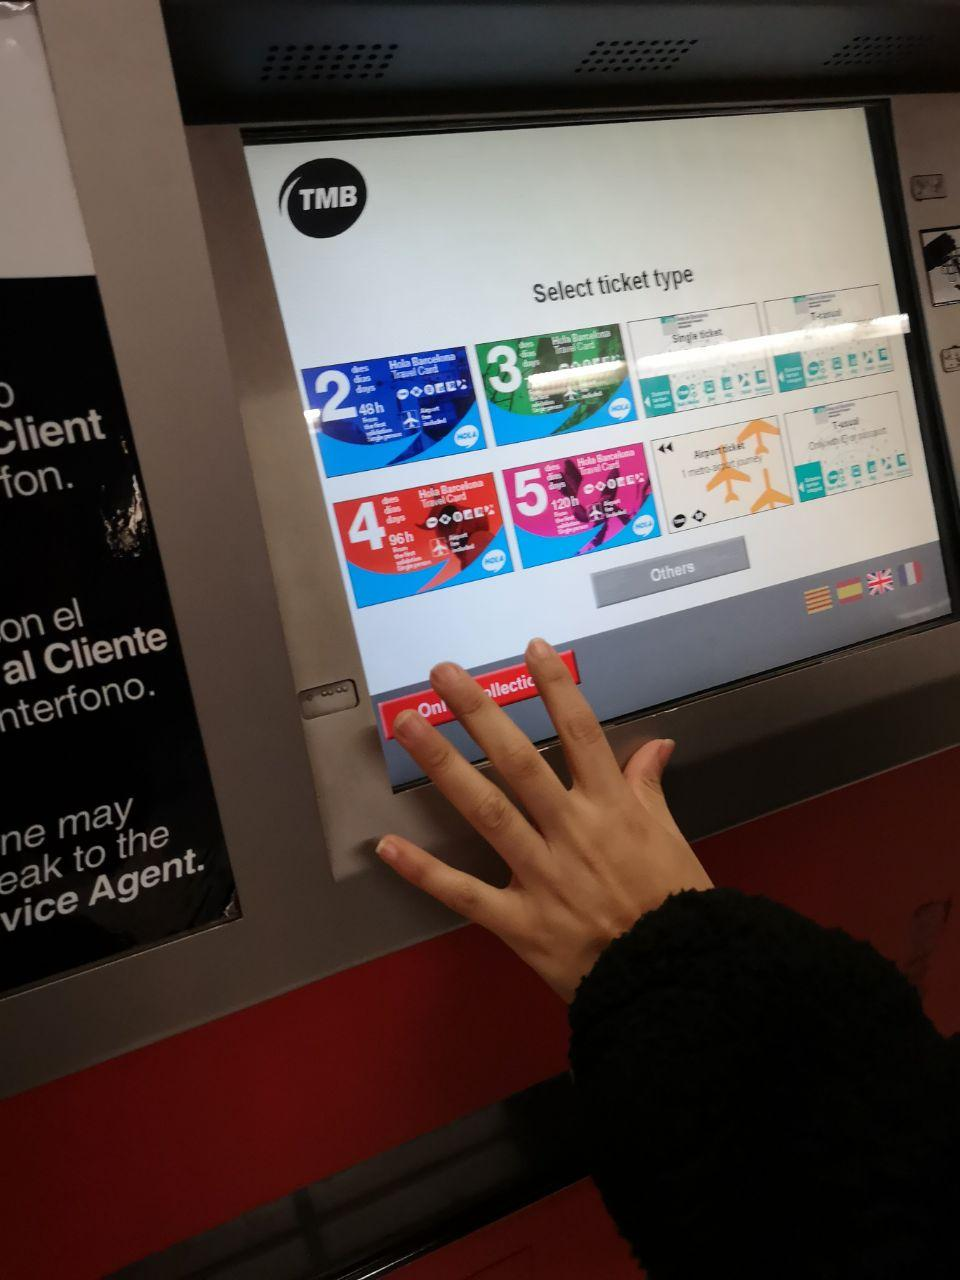
\includegraphics[scale=0.2]{pictures/tickettype.jpg}
	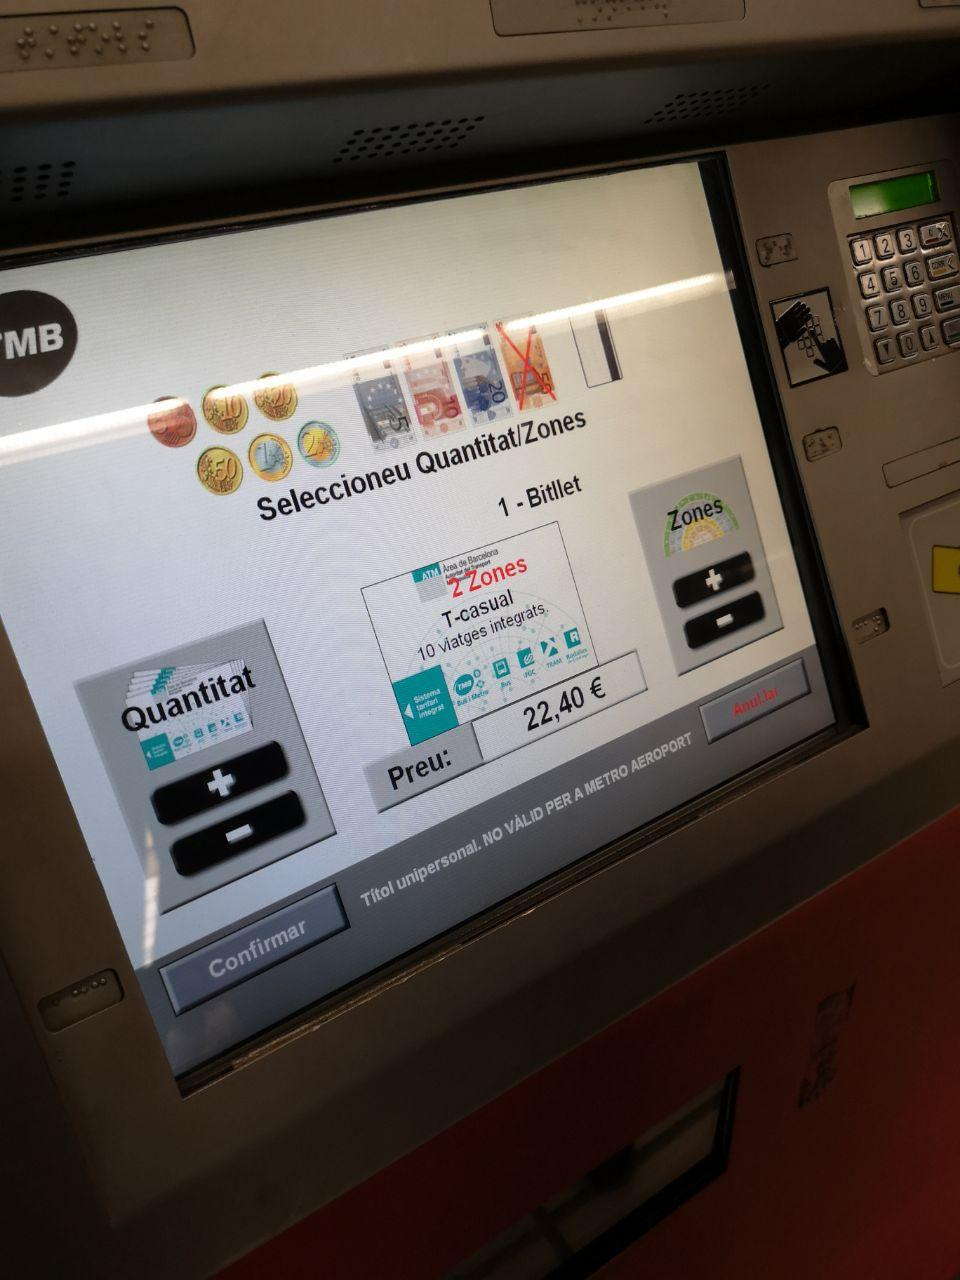
\includegraphics[scale=0.2]{pictures/payment.jpg}
	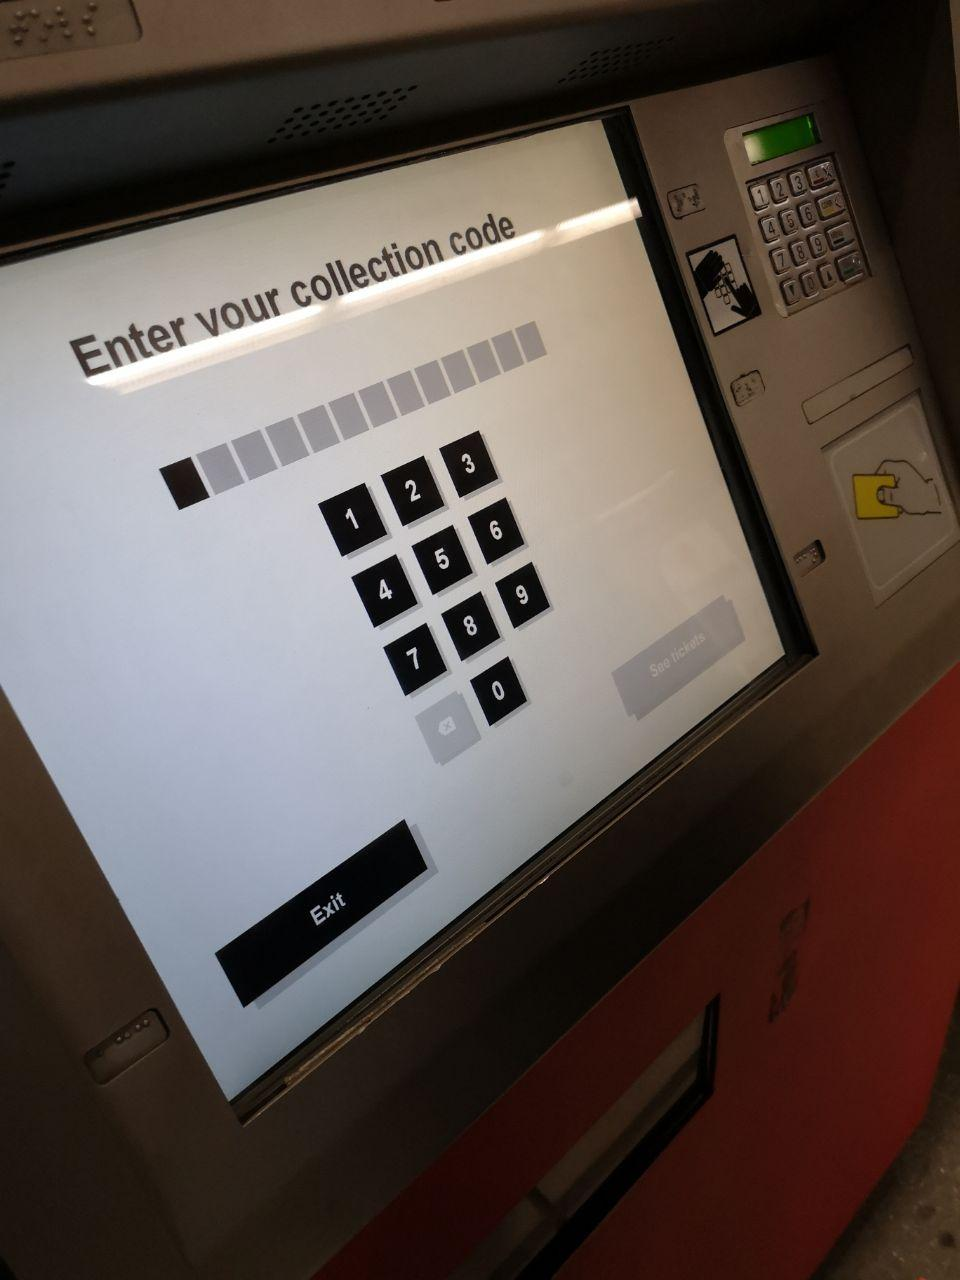
\includegraphics[scale=0.2]{pictures/onlinepurchase.jpg}\\
	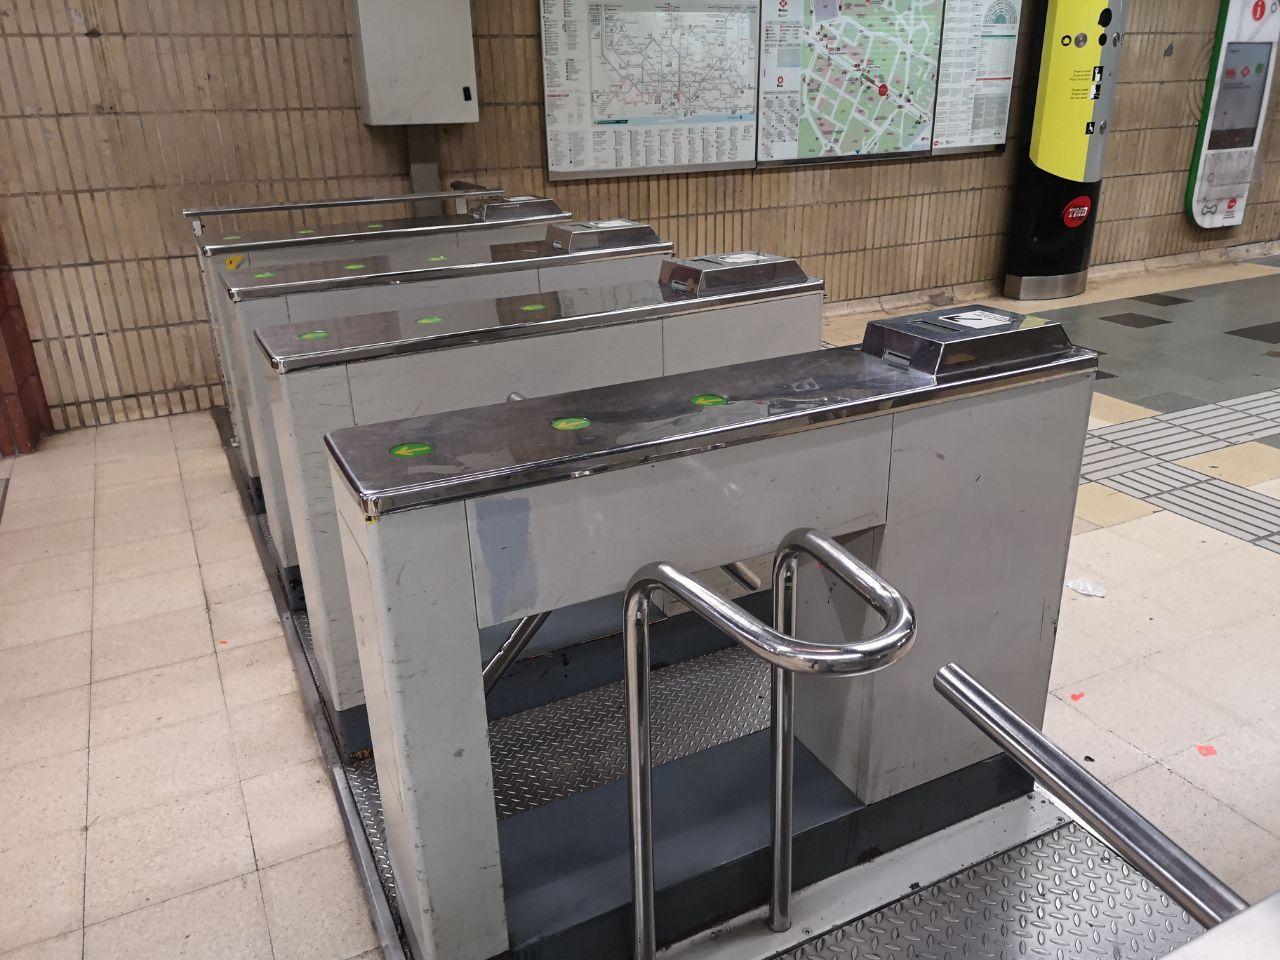
\includegraphics[scale=0.2]{pictures/entrances.jpg}
	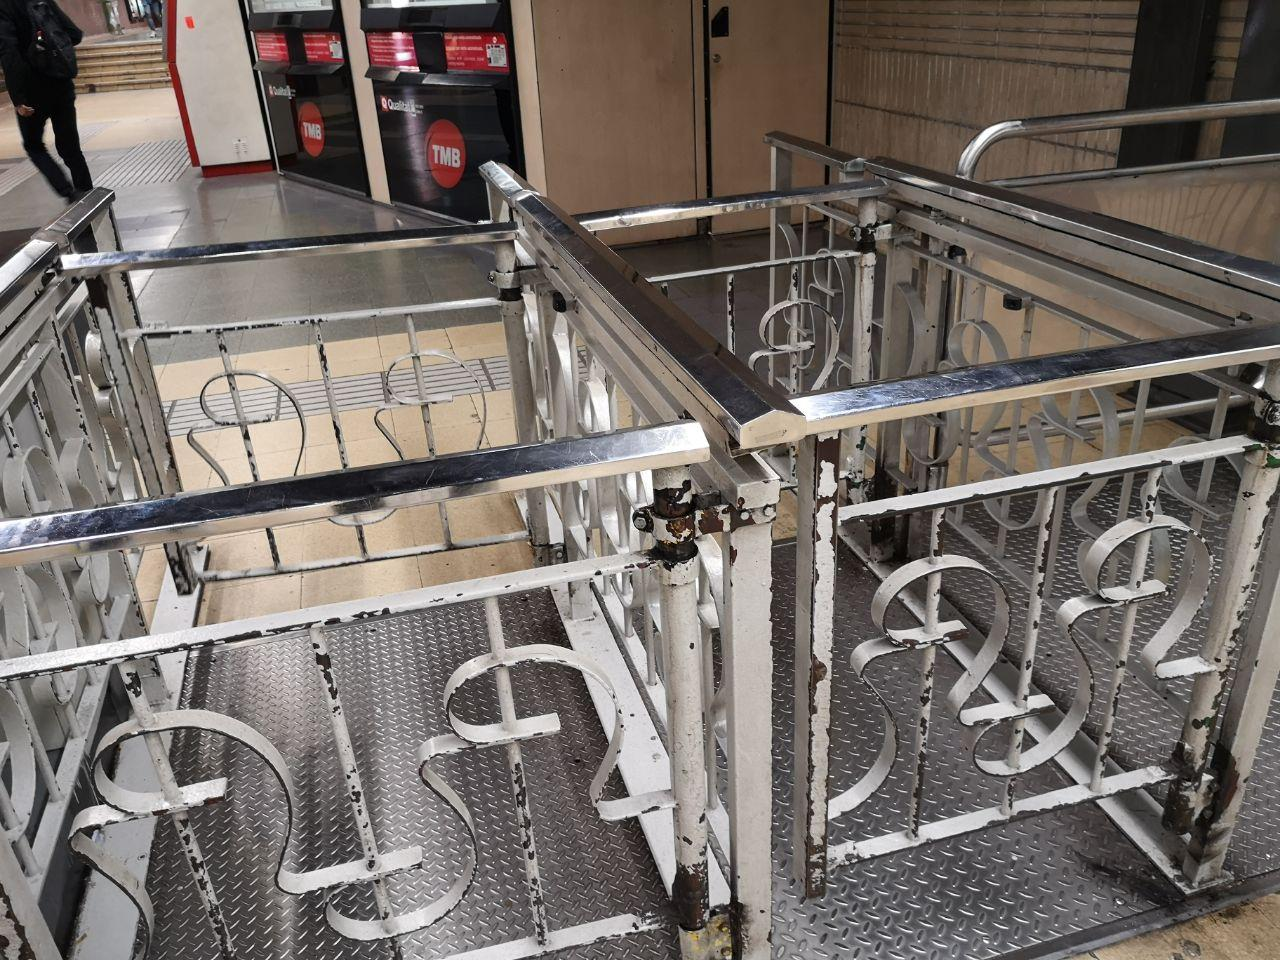
\includegraphics[scale=0.2]{pictures/exits.jpg}

	\subsection*{Oppgave 2 --- Analyse: Sekvens av handlinger}
	\paragraph*{a)}
	En handlingsekvenstabell er en ``to-dimensjonell''-tabell som beskriver hvordan en bruker og en maskin kommuniserer. Langs ``y-aksen'' har vi tidsrommet, og langs ``x-aksen'' har vi i grunnen to spalter, som igjen er hver delt i to.

	Til venstre har vi brukeren, og til h{\o}yre har vi maskinen. Ytterlig til venstre fremkommer alt brukeren gj{\o}r som ikke maskinen ser, og tilsvarende ytterlig til h{\o}yre fremst{\aa}r det maskinen gj{\o}r i bakgrunnen. I de to gjenst{\aa}ende spaltene i midten ser vi hva brukeren og maskinen sier til hverandre.

	I de ytterlige kolonnene er mye informasjon, som muligvis er viktig {\aa} formidle til hverandre.

	Form{\aa}let med denne type tabell er \aa{} kunne analysere hvordan brukere interagerer med maskiner. Vi vil kunne se hvilke forst{\aa}else-problemer som finnes i systemet, for {\aa} dermed ha mulighet til {\aa} forbedre disse.

	\newpage

	\paragraph*{b)}  % tabell

	\begin{tabular}{ | >{\centering}p{10em} || >{\raggedleft}p{10em} | >{\raggedright}p{10em} || >{\centering\arraybackslash}p{10em} | }
	\hline
	\multicolumn{2}{|c|}{Human} & \multicolumn{2}{c|}{Machine} \\\hline
	Environment & {To Machine} & To Human & System design\\\hline\hline
	Approaches machine & & & \\\hline
	 & Presses screen looking for map & & \\\hline
	Looks around &  & & \\\hline
	 & Presses SOS/info button &  & \\\hline
	Silence, waiting &  &  & Calls operator \\\hline
	 &  & Operator voice & \\\hline
	 & Asks for help &  & \\\hline
	 &  & Op: ``Hold on, I will check.'' & \\\hline
	Waits for answer & Acknowledges &  & \\\hline
	 &  & Beeping sounds & Line is on hold. \\\hline
	Confused user &  & Faster beeping sounds & Line is hung up. \\\hline
	Confused user &  &  & Checking \\\hline
	Waiting & Tries to talk to telephone &  & Operator walks towards user \\\hline
	Surprised &  &  & \\\hline
	Talks with operator &  &  & \\\hline
	 &  &  & Operator explains user could press the button to call operator through mobile walkie-talkie again \\\hline
	User understands situation now &  &  &  \\\hline

	\end{tabular}

	\paragraph*{c)}  % analyse av tabell

	Interaksjonen med maskinen er lett s{\aa} lenge man vet hva en gj{\o}r, hva en {\o}nsker, og hvordan systemet fungerer. Hvis ikke man vet hvilken billett man {\o}nsker, og ``bare gj{\o}r det'', oppst{\aa}r det forvirrelser. Det er d{\aa}rlig med informasjon om billetter p{\aa} maskinen, og for {\aa} f{\aa} hjelp vet man ikke helt om det er ``ok'' {\aa} trykke p{\aa} SOS-knappen. N{\aa}r man f{\o}rst velger {\aa} klikke p{\aa} denne vet man ikke hvem man prater med, og man forventer ikke at operat{\o}ren bare legger p{\aa} uten {\aa} si at han kommer til {\aa} fysisk komme for {\aa} hjelpe oss.

	Hadde operat{\o}ren sagt ifra at han legger p{\aa} hadde dette v{\ae}rt mer intuitivt. {\AA} ha to knapper, selv om de i praksis  kunne gjort det samme, for {\aa} separere SOS- og info-hjelpen ville gjort det mer inveterende {\aa} sp{\o}rre etter hjelp. 


	\subsection*{Oppgave 3 --- Øvelse: Oppmerksomhet og distraksjon}

	{\AA} skru av telefonen/nettet er noe jeg er ganske vant med. Jeg bruker telefonen, datamisknen, og b{\ae}rbaren aktivt nesten hver dag for tiden, men (nesten) aldri n{\aa}r jeg er p{\aa} jobb. Hvis noen ringer meg p{\aa} jobben s{\aa} svarer jeg bare dersom det er sjefen, eller andre viktige jobb-kontakter. Hvis ikke det er noen jeg har aktivt lagt til i unntakene til ``Do Not Disturb''-moduset vil jeg ikke f{\aa} notifkasjon f{\o}r etter jeg har tid til {\aa} sjekke meldingene. Jeg anbefaller alle {\aa} ta seg tid til {\aa} sette opp telefonen(e) sine for {\aa} bare f{\aa} de meldingene de er interessert i, og ikke alt annet tull. Tross alt, er det er din telefon, og ikke du som er telefonen sin. 

	{\AA} bruke telefonen som et verkt{\o}y er en positiv ting, s{\aa} lenge man ikke er avhengig av denne. Skru gjerne av telefonen i flere uker om du f{\o}ler den tar kontroll over livet/hverdagen din, siden det betyr at det har g{\aa}tt for langt. Det er fullt mulig {\aa} leve uten telefon selv i dag, der alle andre forventer deg til {\aa} f{\o}lge med p{\aa} lasset. Det handler bare om {\aa} tilpasse seg, ha selvkontroll, og v{\ae}re bevisst om hva en driver med. 

	\subsection*{Oppgave 4 --- Spørsmål til pensum}

	\begin{itemize}
		\item[---] Har det v{\ae}rt noen endring gjennom historien relatert til hva folk foretrekker mellom ``objektive'' og ``ekspressive'' statistikker/m{\aa}linger?
		\item[---] Trenger vi {\aa} m{\aa}le ting objektivt for {\aa} komme til konklusjoner, eller er det nok {\aa} f{\o}lge ``bobler'' som kunstig intelligens kan vise oss?
		\item[---] Kan vi relatere forskjellige m{\aa}leteknikker til forskjellige typer intellgense? Vil noen mennesker ha det lettere for {\aa} forst{\aa} ting om vi presenterer informasjon p{\aa} en ``strippet'' og ``tall-orientert'' m{\aa}te enn andre? 
	\end{itemize}

	\subsection*{Oppgave 5 --- Refleksjon}

	Den mest informative delen ved denne obligen var delen om m{\aa}linger. Jeg tenker ofte p{\aa} forskjellige m{\aa}ter {\aa} ``lese og skrive'' informasjon, s{\aa} jeg synes det er spennende {\aa} l{\ae}re om forskjellige m{\aa}ter man kan presentere eller samle samme informasjonen/virkeligheten. Likevel synes jeg det var spennende {\aa} gj{\o}re observasjonsdelen, selv om jeg ikke f{\o}lte jeg observerte nok deltagere for {\aa} f{\aa} noe generell informasjon om hvordan brukere generelt anvender systemet. Jeg tror det ville v{\ae}rt mer effektiv {\aa} gj{\o}re en eller flere sp{\o}rreunders{\o}kelser.

	{\AA} kunne sammenligne systemet her i Barcelona versus systemet i Norge tror jeg har v{\ae}rt den  mest nyttige delen ang{\aa}ende forskjellige systemet, siden jeg merker forskjellen p{\aa} hvordan folk bruker systemene her med tanke p{\aa} hvordan disse er lagt opp. Jeg tror ogs{\aa} at {\o}konomien og kulturen definerer hvordan systemene m{\aa} v{\ae}re for {\aa} v{\ae}re effektive. Det finnes intet perfekt system som fungerer overalt. Systemene m{\aa} tilpasses folket der det blir brukt.

\end{document}